% !TeX spellcheck = en_GB
\section{Preface}\label{Preface}
In the software world, or more specific, the Java enterprise world, developers tend to abstract access to data in a way that components are interchangeable. A perfect example for such an abstraction is the usage of Object Relational Mappers (ORM). The database specifics are mostly irrelevant to the average developer and the need for native SQL is brought down to a minimum. This makes the switch to a different relational database system (RDBMS) easier in the later stages of a product's life cycle.
\\\\
The Java Persistence API (JPA) went even further by standardising ORMs. First conceived in 2006 \cite{needed}, it is now the de-facto standard for Object Relational Mappers in Java. The developer doesn't need to know which specific ORM is used in the application, as all the database queries are written against a standardized query API and therefore portable. This means that not only the database is interchangeable, but even the specific ORM, it is accessed by, is as well.
\\\\
However, this does not mean that all JPA implementations ship with the same features. While all of them are JPA compliant (apart from minor bugs), some ship with additional modules to enhance their capabilities. A perfect example for this is the Hibernate Search API aimed at Hibernate ORM users: Nowadays, even small applications like online shops need enhanced search capabilities to let the user find more results for a given input.
\\\\
This is not something a regular RDBMS excels at and Hibernate Search comes into use: It works atop the Hibernate ORM/JPA system and enables the developer to index the domain model for searching. It's not only a mapper from JPA entities to a search index, but also keeps the index up-to-date if something in the database changes.
\\\\
\begin{figure}[ht]
	\centering
	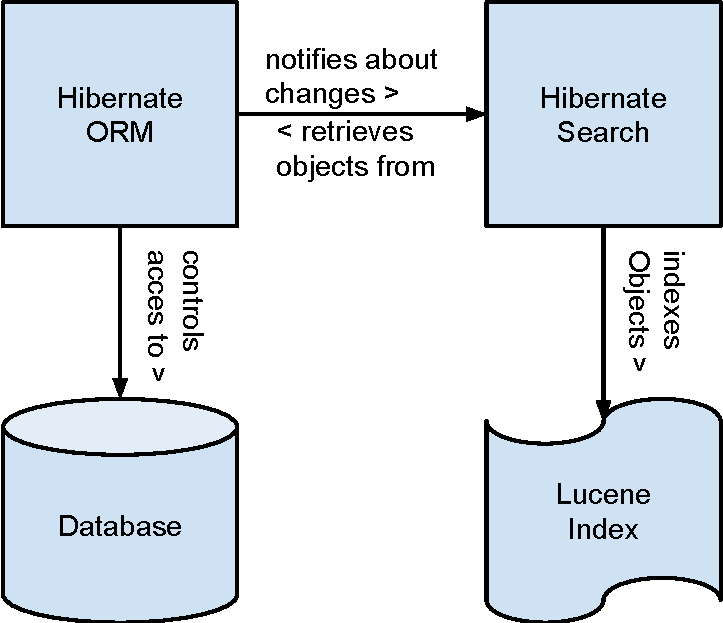
\includegraphics[scale=0.5]{images/hibernate_search_hibernate_schema.pdf}
		\caption{Hibernate Search with Hibernate ORM}
		\label{fig1}
\end{figure}
\\
Hibernate Search, which is based on the powerful Lucene search toolbox, is a separate project in the Hibernate family and is using a lot of JPA interfaces in its codebase and aims to provide a JPA "feeling" in its API. However, this does not mean that it is compatible with other JPA providers than Hibernate ORM (apart from Hibernate OGM, the NoSQL JPA mapper of the family).
\\\\
\begin{figure}[ht]
	\centering
	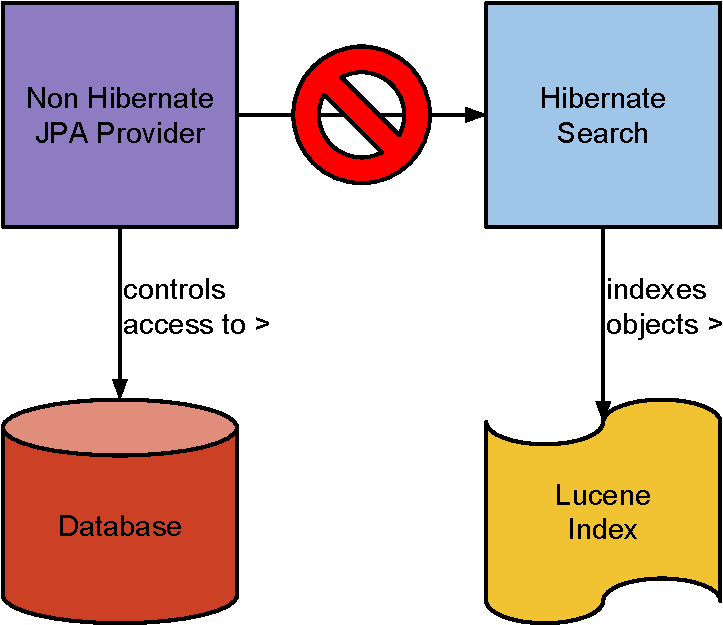
\includegraphics[scale=0.5]{images/hibernate_search_any_jpa_problem_schema.pdf}
	\caption{Hibernate Search's incompatibility with other JPA implementations}
	\label{fig2}
\end{figure}
\\
While using Hibernate Search obviously is beneficial for Hibernate ORM applications, not all developers can bind themselves to a specific JPA implementation in their application. For some, the ability to change the it is of strategic important, for others it is just sheer preference to use a different JPA implementation.
\\\\
Currently these developers have to resort to using different full text search systems like native Lucene, ElasticSearch or Solr. While this is always a viable option, for some applications Hibernate Search would be a much better suit because of it's design with a entity structure in mind and the automatic index updating feature, if it just were compatible with generic JPA.
\\\\
When investigating Hibernate Search's project structure \cite{source-code-git}, we see that the only module apart from some server-integration modules that depends on any ORM logic is "hibernate-search-orm". The modules that contain the indexing engine, the replication logic, alternative backends, etc. are completely independent from any ORM logic. This means, that we can reuse most of the codebase for a generic version of Hibernate Search.
\\\\
In this thesis we will show how such a generic version can be built. We will look at how Hibernate Search's engine can be reused. Then, we will write a standalone version of this engine and finally integrate it with generic JPA.

\pagebreak

\section{Overview}\label{Introduction}

\subsection{An overview of different database paradigms}

\textcolor{red}{das hier anders}

When it comes to persisting data in applications, nowadays there exist a lot of different
paradigms that one has to choose from. Following is a short explanation for the two currently most used ones.

\subsubsection{relational databases}

\subsubsection{NoSQL databases}

\subsection{Object Relational Mappers}

While the NoSQL approach is undeniably rising in popularity, the demand for
relational solutions is still unmatched, as it has been used and has proven itself in practice
for many years now.
\\\\
Nowadays, many popular languages like Java, C\#, etc. are object-oriented.
While SQL solutions for querying relational databases exist for these languages, the user either has to work with the rowsets manually or convert them into custom data access objects. Both approaches include a lot of manual work.
\\\\
This is where Object Relational Mappers (ORM) come into use. They map tables to entity-classes and
enable users to write queries against these classes instead of tables. This is especially useful if used
in big software products as not all programmers have to know the exact details of the underlying database. The database system could even be completely replaced for another (provided the ORM supports the specific RDBMS), with the business logic not changing a bit.

\subsubsection{JPA}

The first version of the JPA standard was released in May 2006. From then on it rose to probably the most commonly used persistence API for Java. While mostly known for standardizing relational database mappers (ORM), it supports other concepts like NoSQL or XML storage as well. However, when talking about JPA in this thesis we will be focusing on the relational aspects of it. Currently, the newest version of this standard is 2.1.\footnote{Wikipedia on Java Persistence API, see~\cite{wiki_jpa}}.
\\\\
Some popular relational implementations are:
\begin{itemize}
	\item Hibernate ORM (JBoss)
	\item EclipseLink (Eclipse foundation)
	\item OpenJPA (Apache foundation)
\end{itemize}
\textcolor{red}{vll Beispiel für eine einfache Beziehung, ER-Modell vs. gemappte Klasse}
\\\\
Using the standardized JPA API over any native ORM API has one really interesting benefit:
The specific JPA implementation can be swapped out. This is particularily important if you are working in a Java EE environment. Java EE itself is a specification for platforms, mostly Web-servers (JPA is part of the Java EE spec).\footnote{Wikipedia on Java EE, see~\cite{wiki_java_ee}} Many Java EE Web-servers ship with a bundled JPA implementation that they are optimized for. This means that if a user switches servers, he/she is also likely to swap out the JPA implementor. If everything in the application is written in a JPA compliant way, the user will then generally not run into many problems related to this switch.

\subsection{Fulltext search}

Conventional relational databases are good at retrieving and querying structured data. But if one wants to build a search engine atop a domain model, most RDBMS will only support the SQL-LIKE operator:\\

\lstset{language=sql}
\begin{lstlisting}[frame=htrbl, label={lst:result2}]
SELECT book.id FROM book WHERE book.name LIKE %name%;
\end{lstlisting}
While this might be enough for some applications, this wildcard query doesn't support features a good search engine would need, for example:

\begin{itemize}
	\item fuzzy queries (variations of the original string will get matched, too)
	\item phrase queries (search for a specified phrase)
	\item regular expression queries (matches are determined by a regular expression)
\end{itemize}
There may exist some RDBMS that support similar query-types, but in the context of using a ORM we would then lose the ability to switch databases since we require specific features not every RDBMS supports.
\\\\
Fulltext search engines can be used to complement databases in this regard. They are not intended to be replacing the database, but to add additional functionality by indexing the data that is to be searched in a more sophisticated way. We will now take a look at some of the most popular available options for Java developers while focusing on their usage, features, the pros and cons of using them, and compatibility with the JPA standard.

\subsubsection{Lucene}

\textcolor{red}{mention current version for each of these?}

\begin{quote}
Apache LuceneTM is a high-performance, full-featured text search engine library written entirely in Java. It is a technology suitable for nearly any application that requires full-text search, especially cross-platform.\footnote{official Lucene website, see~\cite{lucene_apache_org}}
\end{quote}
Lucene serves as the basis for most fulltext search engines written in Java. It has many different utilties and modules aimed at search engine developers. However, it can be used on its own as well.

\paragraph{Index structure}
Lucene uses an \textbf{inverted index} to store data. This means that instead of storing texts mapped to the words contained in them, it works the other way around. All different words (or terms) are mapped to the texts they occur in.\footnote{Lucene basic concepts, see~\cite{lucene_basic_concepts}} Also, before anything can be searched using Lucene, it has to be added to the the index first.

\paragraph{Concepts} Lucene has its own set of concepts that need to be discussed first before we can take a look at it's usage. Following is the explanation of the most important ones.

\subparagraph{Documents}
Documents are the data-structure Lucene stores and retrieves from the index. A index can contain zero or more Documents. Documents are added to the index with an IndexWriter and retrieved via an IndexReader/IndexSearcher.

\subparagraph{Fields}
A Document consists of at least one field. Fields are basically tuples of key and value. They can be stored (can be retrieved from the index) and/or indexed (can be searched on).

\subparagraph{Analyzers}
Before documents get indexed, their fields are analyzed first. Analysis is the process of modifying the input in a manner such that it can be searched upon (stemming, tokenization, ...). In Lucene this is done by special classes called Analyzers.

\paragraph{Usage - Indexing}
We will now take a look at how data is indexed in Lucene. In the following example we consider the data to be already present in form of a List of objects of the class 'Text' and concentrate on the Lucene usage itself.
\\\\
\textcolor{red}{Beispiel für Lucene usage hier, }

\paragraph{Usage - Searching}
Searching\\\\
\textcolor{red}{Beispiel für Lucene usage hier, }

\paragraph{Features}
Lucene is probably the most complete toolbox to build a search-engine from.

\paragraph{Pros and Cons}

\paragraph{Compatibility with JPA}
By design, Lucene out of the box is not very compatible with the JPA standard. For one, the flat document structure forces the user to de-normalize the entity model before indexing. Secondly, since every search-relevant change in the database should be reflected in the index, it must be kept up to date. When using Lucene, this has to be done completely manually as it natively doesn't have any integration with databases.

\subsubsection{Solr}

\subsubsection{ElasticSearch}

\subsubsection{Hibernate Search}

\textcolor{red}{some kind of conclusion with a table of features. -> Hibernate Search, aber mit dem Problem von Kompatibilität mit Non Hibernate ORM, mention Compass?}

\subsection{aims of this thesis}
